\documentclass[12pt,a4paper]{article}
\usepackage{geometry}
\geometry{left=2.5cm,right=2.5cm,top=2.0cm,bottom=2.5cm}
\usepackage[english]{babel}
\usepackage{amsmath,amsthm}
\usepackage{amsfonts}
\usepackage{bm}
\usepackage[longend,ruled,linesnumbered]{algorithm2e}
\usepackage{siunitx}
\usepackage{fancyhdr}
\usepackage{ctex}
\usepackage{array}
\usepackage{listings}
\usepackage{color}
\usepackage{graphicx}
\usepackage{float}
\usepackage{caption}
\usepackage{longtable}

\begin{document}
    \title{\heiti{《机器学习》课程第 {$3$} 次作业}}
    \date{}
    \author{姓名:\underline{刘哲}~~~~~~学号:\underline{2022103691}~~~~~~}
    \maketitle
    \section{\heiti{Auto}}
    \vspace{10pt}
    \subsubsection*{a}
    Auto数据集中的所有变量的散点图矩阵如下:
    \begin{figure}[H]
        \centering
        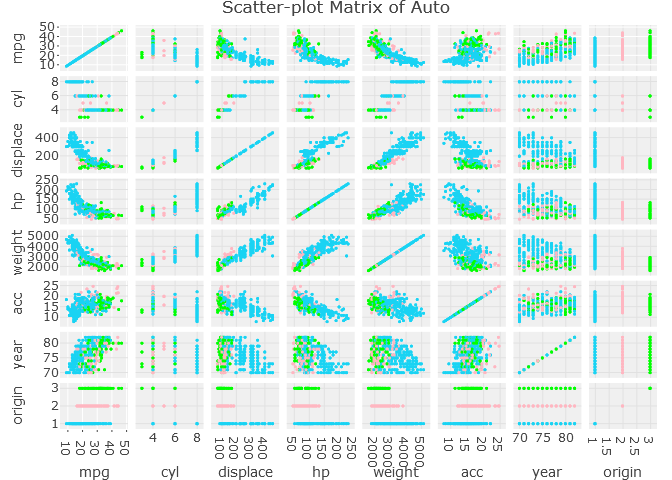
\includegraphics[scale=0.65]{Splom.png}
    \end{figure}
    其中,mpg是每加仑汽油英里数,cyl是气缸数,displace是发动机排量,hp是发动机马力,
    weight是车重,acc是60英里加速时间,year是出品年份,origin是汽车原产地。
    \subsubsection*{b}
    排除车名变量,其余各变量之间的相关系数矩阵为
    \begin{longtable}{c|cccccccc}
        \hline
         & mpg & cyl & displace & hp & weight & acc & year & origin\\
        \hline
        mpg & 1 & -0.7776 & -0.8051 & -0.7784 & -0.8322 & 0.4233 & 0.5805 & 0.5652\\
        % \hline
        cylinders & -0.7776 & 1 & 0.9508 & 0.8430 & 0.8975 & -0.5047 & -0.3456 & -0.5689\\
        % \hline
        displacement & -0.8051 & 0.9508 & 1 & 0.8973 & 0.9330 & -0.5438 & -0.3699 & -0.6145\\
        % \hline
        horsepower & -0.7784 & 0.8430 & 0.8973 & 1 & 0.8645 & -0.6892 & -0.4164 & -0.4552\\
        % \hline
        weight & -0.8322 & 0.8975 & 0.9330 & 0.8645 & 1 & -0.4168 & -0.3091 & -0.5850\\
        % \hline
        acceleration & 0.4233 & -0.5047 & -0.5438 & -0.6892 & -0.4168 & 1 & 0.2903 & 0.2127\\
        % \hline
        year & 0.5805 & -0.3456 & -0.3699 & -0.4164 & -0.3091 & 0.2903 & 1 & 0.1815\\
        % \hline
        origin & 0.5652 & -0.5689 & -0.6145 & -0.4552 & -0.5850 & 0.2127 & 0.1815 & 1\\
        \hline
    \end{longtable}
    \subsubsection*{c}
    以mpg作为响应变量,进行多元线性回归。由于origin是分类变量,将其转换为哑变量(American, European)。
    其中,(1, 0)表示origin=1,即汽车原产地为American;(0, 1)表示origin=2,即汽车原产地为European;(0, 0)表示origin=3,即汽车原产地为Janpanese。
    回归结果如下:
    \begin{figure}[H]
        \centering
        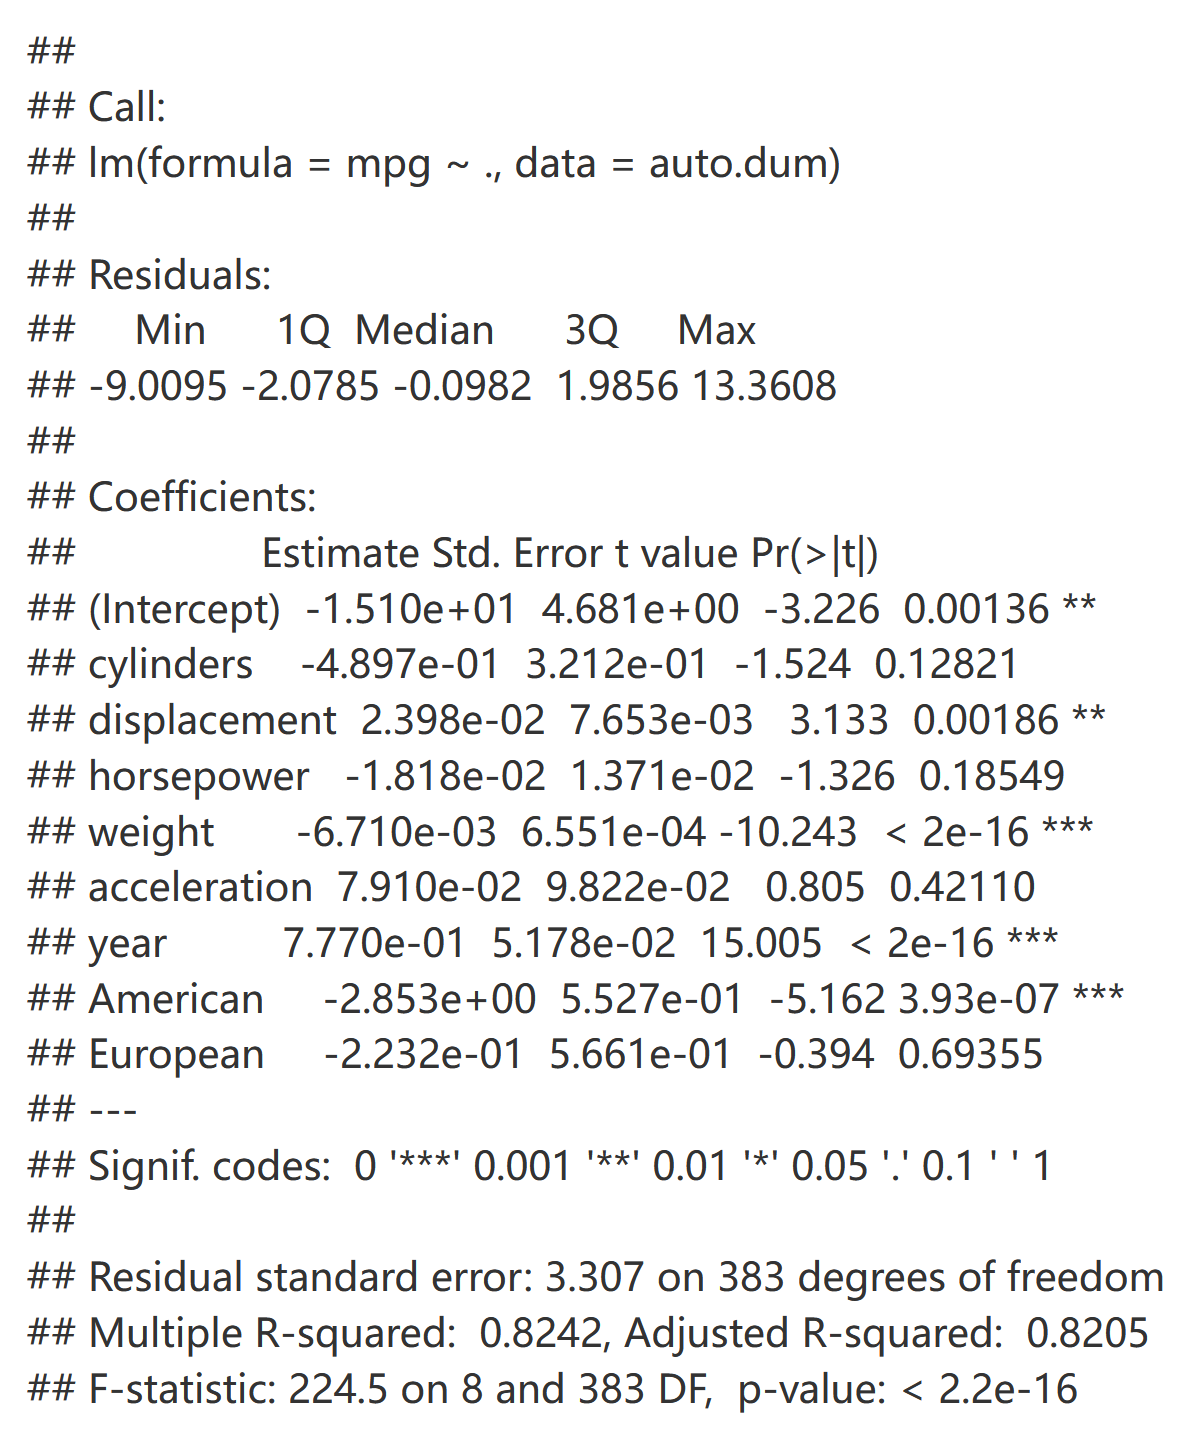
\includegraphics[scale=0.3]{Auto_LR.png}
    \end{figure}
    由回归方程F检验的p-value极小可知,回归方程显著,但并不是所有预测变量都与响应变量具有显著相关性。
    其中预测变量displacement、weight、year、American和截距项的回归系数显著,说明其与mpg在统计上具有显著关系。\par
    发动机排量(displacement)具有正回归系数,表明发动机排量越大,mpg越大;车重(weight)具有负回归系数,表明汽车越重,mpg越小;
    出品年份(year)具有正回归系数,表明新款汽车的mpg更大,汽车的mpg具有逐年上升的趋势;哑变量American具有负回归系数,表明美国产汽车的mpg更小。
    \subsubsection*{d}
    多元线性回归的诊断图如下:
    \begin{figure}[H]
        \centering
        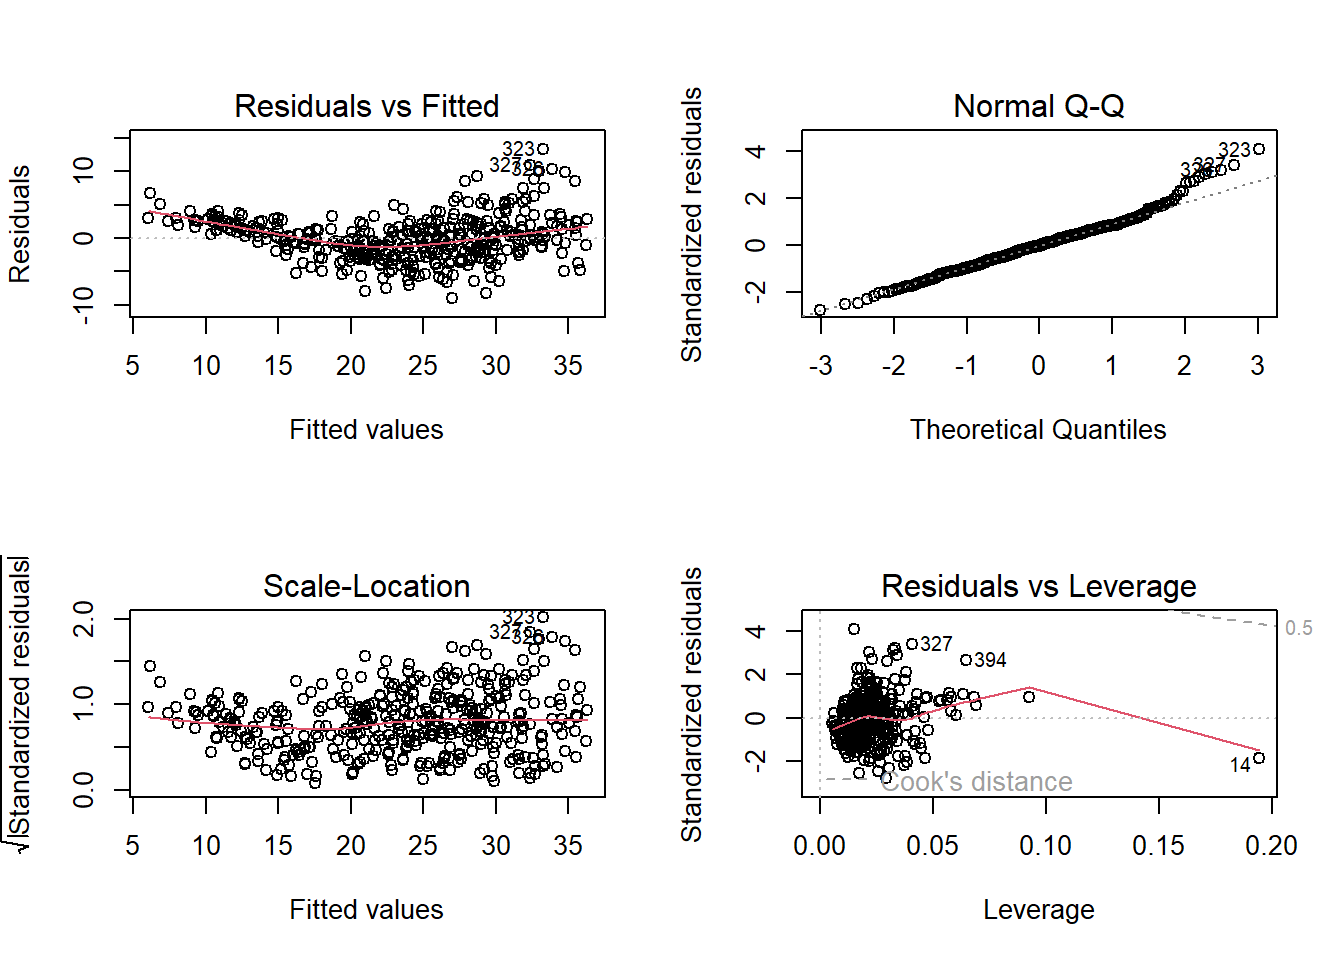
\includegraphics[scale=0.75]{Diagnostic.png}
    \end{figure}
    由Residuals图可以看出,残差点基本上在一条水平直线附近,但当拟合值较大时,残差点变得更加分散,出现大量离群点。
    Normal Q-Q图基本上形成了一条直线,表明拟合残差满足正态性。
    Scale-Location图中出现一条水平直线,表明残差沿着预测值的范围平均分布,符合同方差性假设。
    Leverage图显示了离群点对回归的影响,因为图中几乎看不到Cook距离线,说明所有样本点都在Cook距离线内部,表明不存在异常高杠杆作用的点,离群点对回归几乎没有影响。
    \subsubsection*{e}
    使用逐步选择法建立回归模型,结果如下:
    \begin{figure}[H]
        \centering
        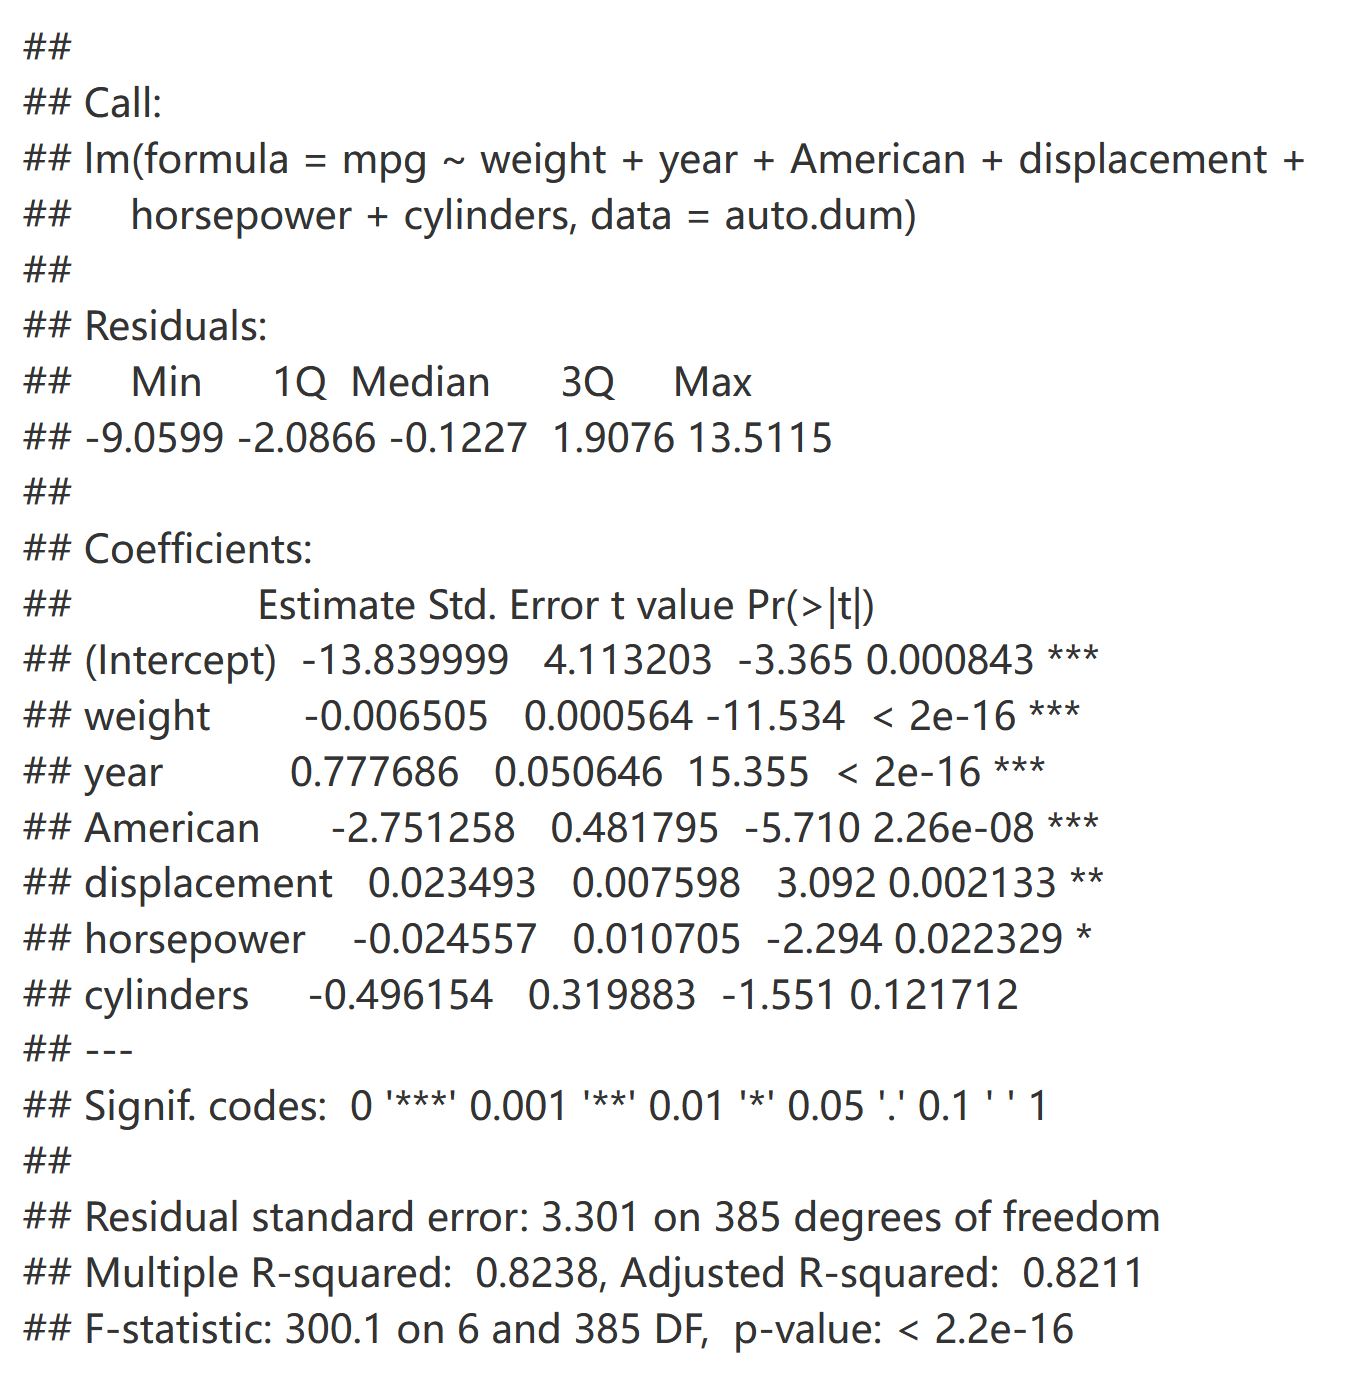
\includegraphics[scale=0.3]{StepwiseAuto.png}
    \end{figure}
    根据回归系数的显著性,选择最佳变量weight、year、American建立回归模型,结果如下:
    \begin{figure}[H]
        \centering
        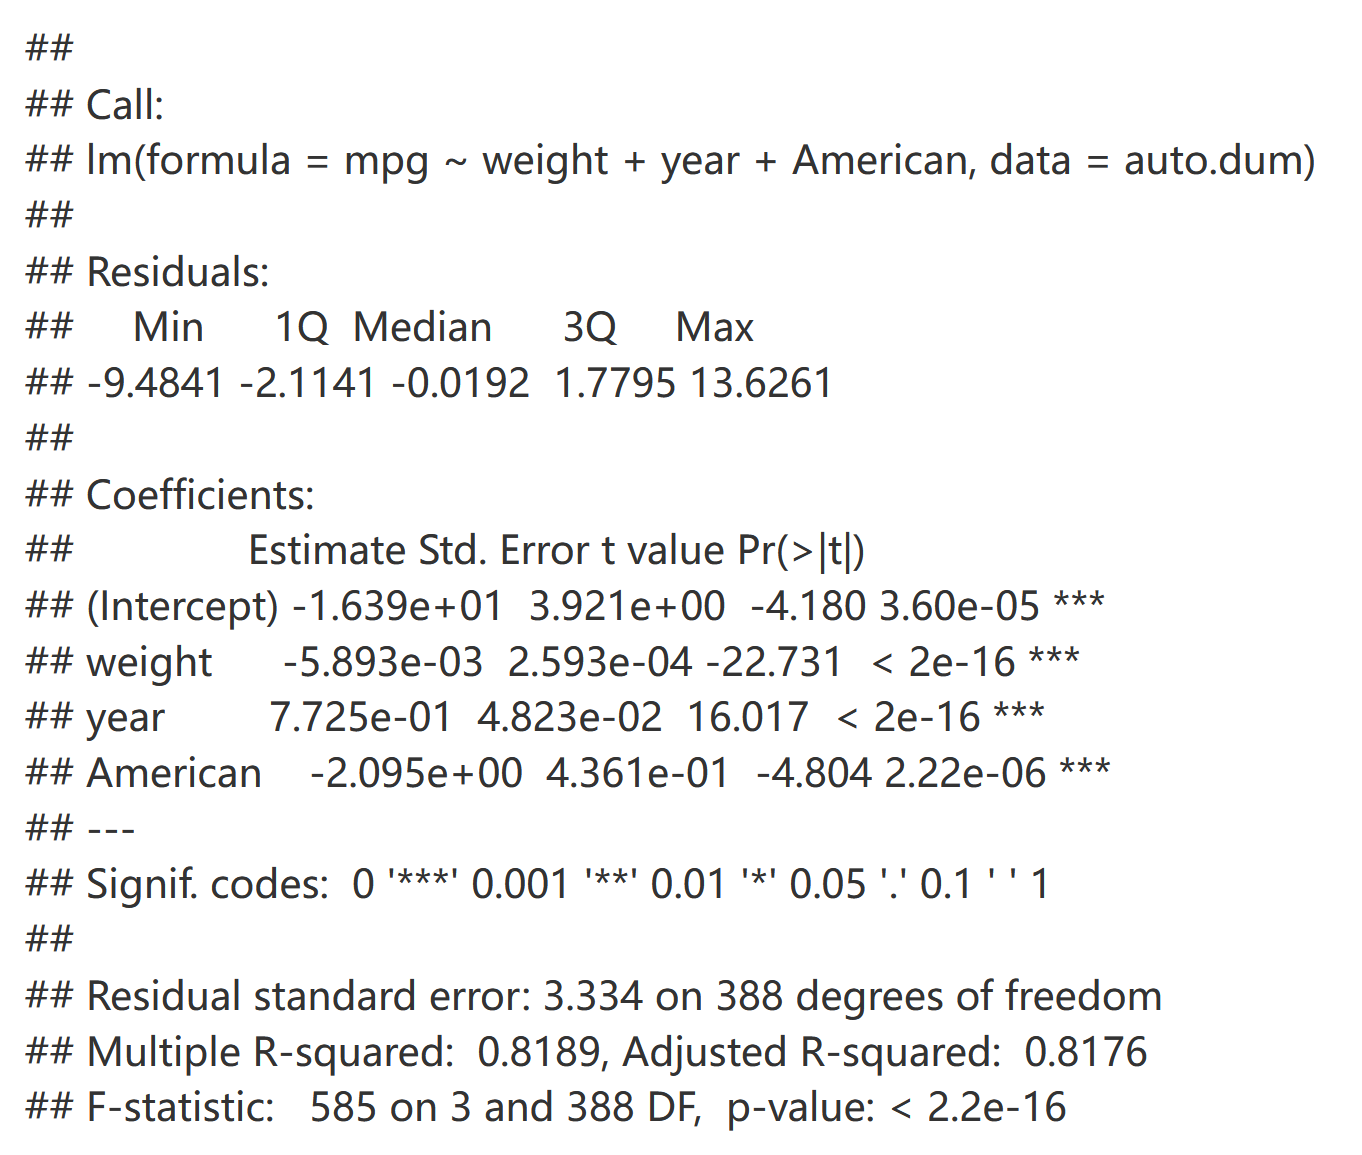
\includegraphics[scale=0.3]{Stepwise3.png}
    \end{figure}
    使用连续正交法得到每个预测变量在排除其他预测变量的干扰后,对响应变量的相关系数。
    \begin{longtable}{c|c}
        \hline
        var & coef\\
        \hline
        \textbf{cylinders} & \textbf{-3.5581}\\
        \hline
        displacement & -0.0511\\
        \hline
        horsepower & -0.0599\\
        \hline
        weight & -0.0053\\
        \hline
        acceleration & -0.0291\\
        \hline
        \textbf{year} & \textbf{0.7534}\\
        \hline
        \textbf{American} & \textbf{-2.7469}\\
        \hline
        European & -0.2232\\
        \hline
    \end{longtable}
    系数绝对值的大小代表了对应预测变量对响应变量的影响大小,因此选择最佳变量cylinders、year、American建立回归模型,结果如下:
    \begin{figure}[H]
        \centering
        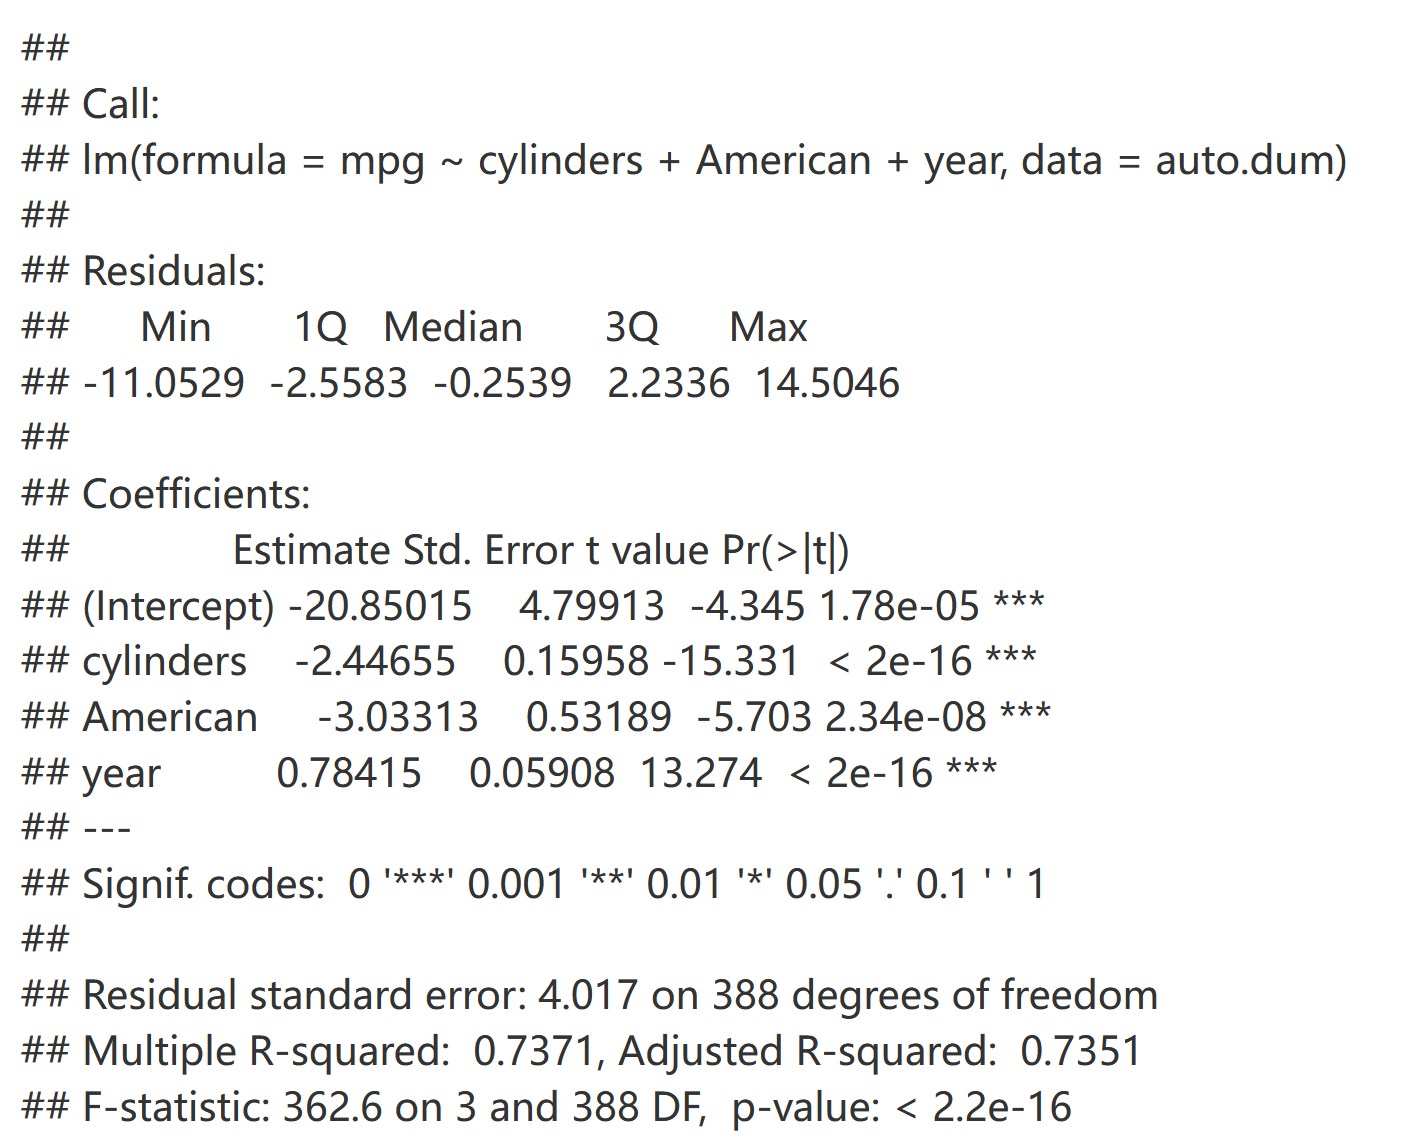
\includegraphics[scale=0.3]{Ortho3.png}
    \end{figure}
    比较两个回归模型,根据逐步选择法筛选出变量,由此建立的回归模型具有更大的$R^2$和调整$R^2$,
    认为使用变量weight、year、American作为预测变量建立的回归模型具有更优的性能。
    \section{\heiti{Hitters}}
    \vspace{10pt}
    \subsubsection*{a}
    Hitters 数据集中有 59 名球员的 Salary 变量为空,不利于后续基于 Salary 的分析研究,故将这部分球员删去。\par
    将剩余样本的 Salary 变量排序,其散点图如下:
    \begin{figure}[H]
        \centering
        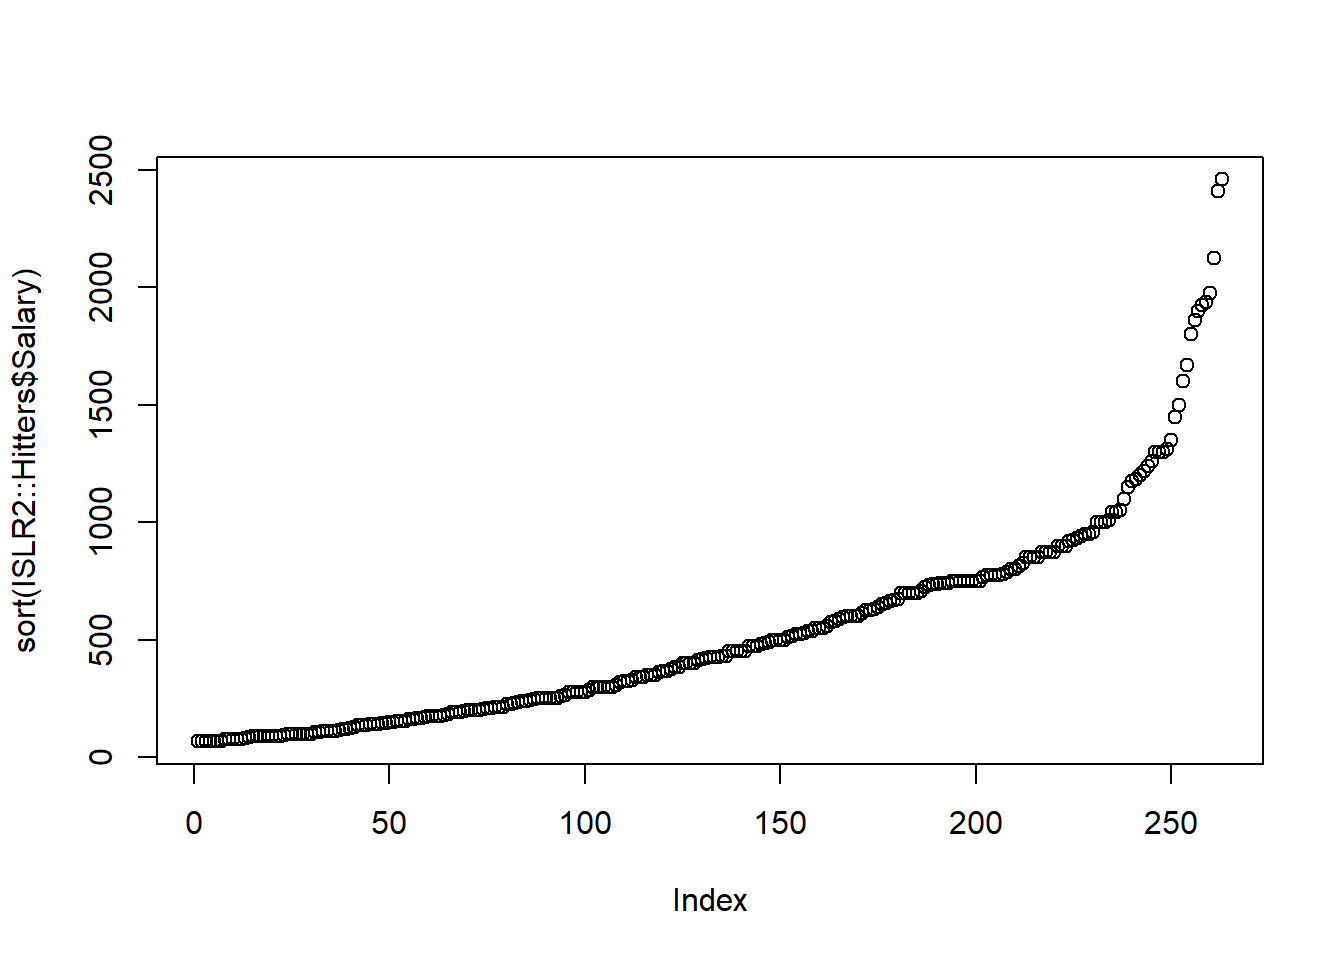
\includegraphics[scale=0.65]{Salary.png}
    \end{figure}
    选取阈值为 500,即认为 Salary 大于 500 的击球手属于高薪球员,记为1;其余则属于低薪球员,记为0。
    数据集中球员薪资水平的分布如下:
    \begin{longtable}{c|c|c}
        \hline
        Salary & 1 & 0\\
        \hline
        n & 112 & 151\\
        \hline
    \end{longtable}
    属于高薪和低薪的球员数量相近,有利于建立二分类模型。
    \subsubsection*{b}
    使用逐步选择法建立回归模型,结果如下:
    \begin{figure}[H]
        \centering
        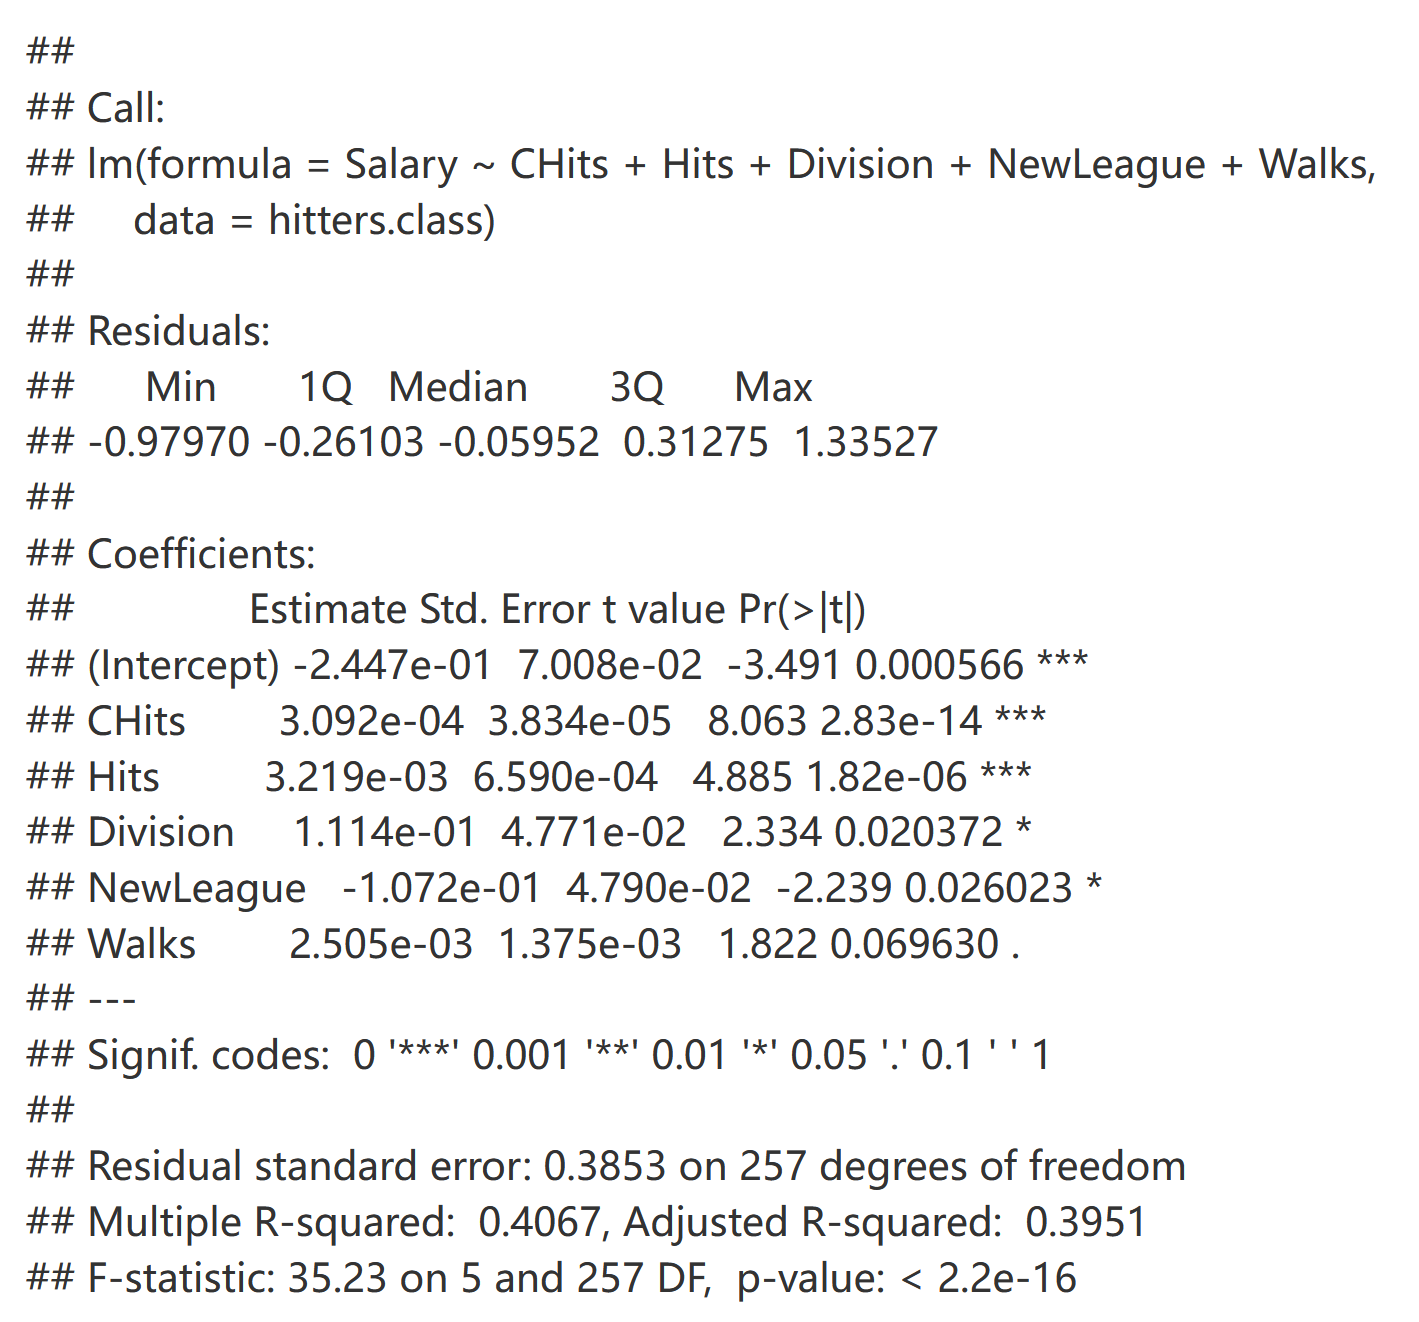
\includegraphics[scale=0.3]{StepwiseHitters.png}
    \end{figure}
    选择其中显著性最高的两个变量 CHits 和 Hits 建立 logistic 回归模型,结果如下:
    \begin{figure}[H]
        \centering
        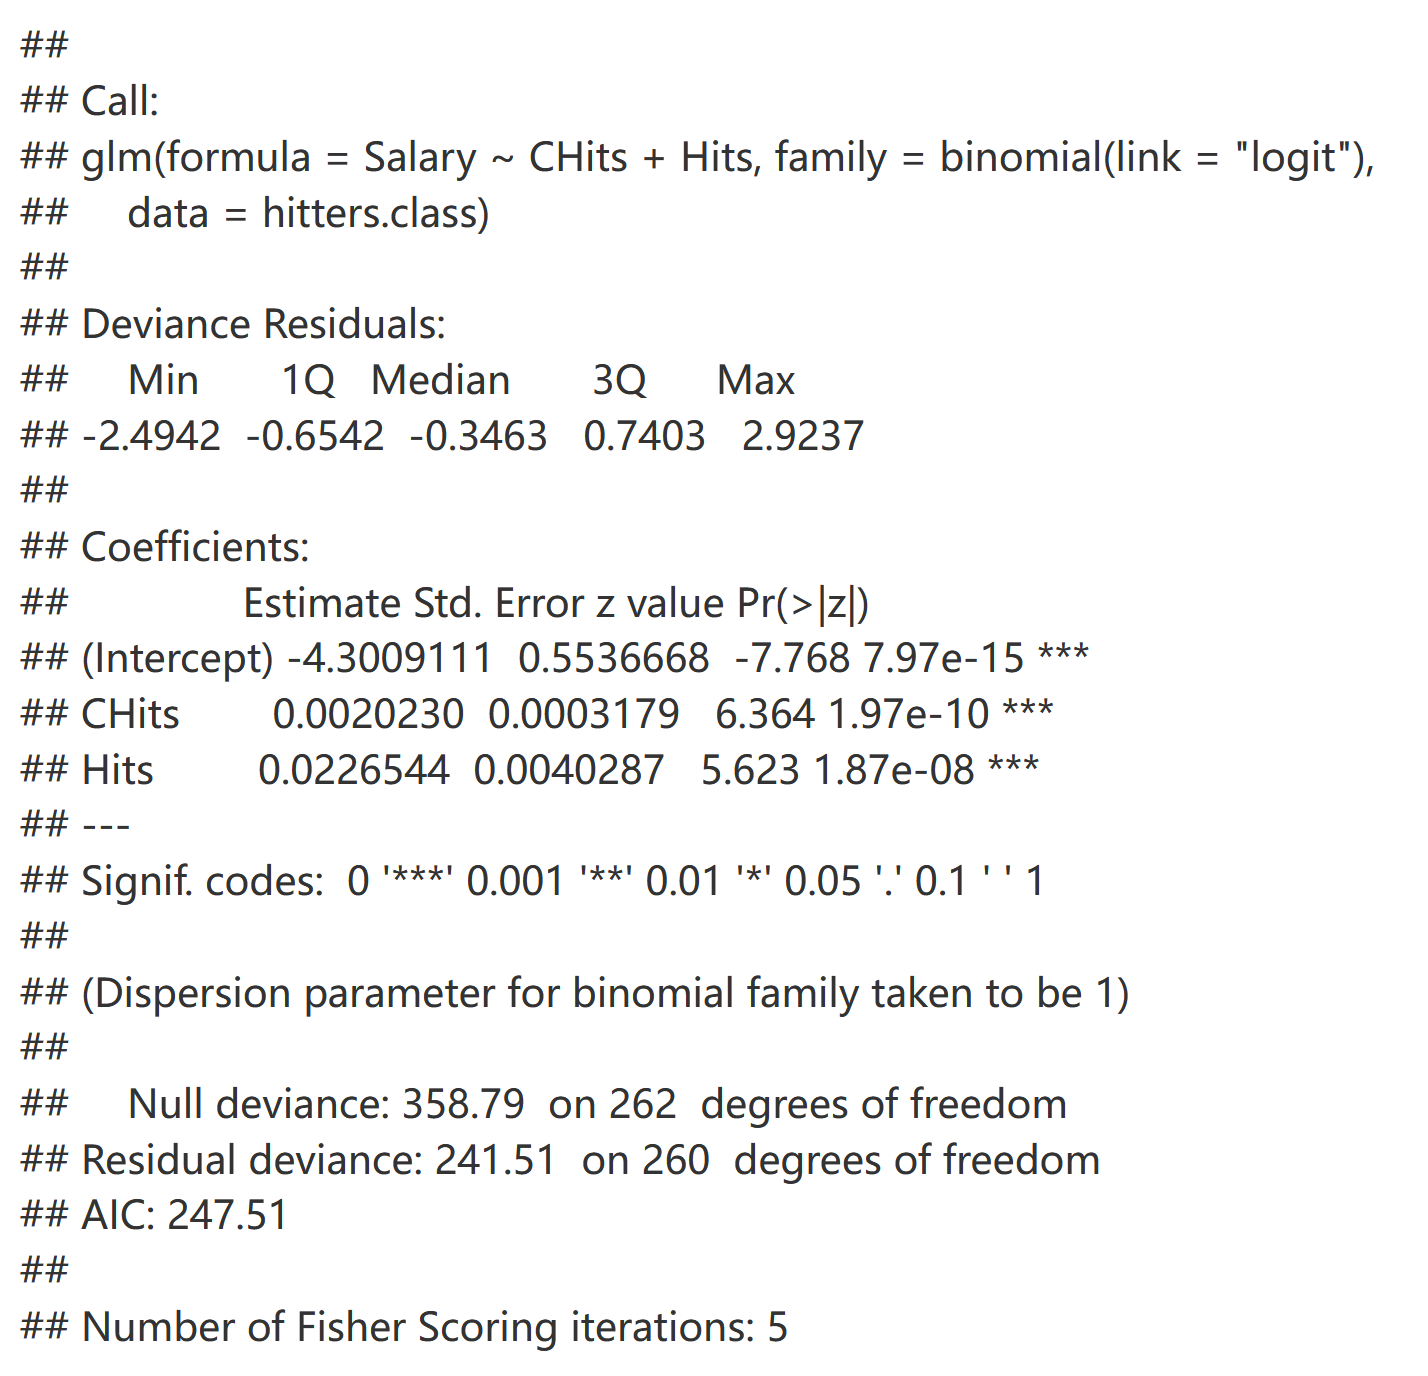
\includegraphics[scale=0.3]{Logistic.png}
    \end{figure}
    显然,logistic 回归模型的参数均显著,且模型准确率为0.8137。
    \subsubsection*{c}
    共有49个球员的薪资水平被预测错误,其中将低薪球员预测成高薪球员的有20个,将高薪球员预测成低薪球员的有29个。
    对预测错的样本进行核密度估计,两个变量 CHits 和 Hits 的分布图如下:
    \begin{figure}[H]
        \centering
        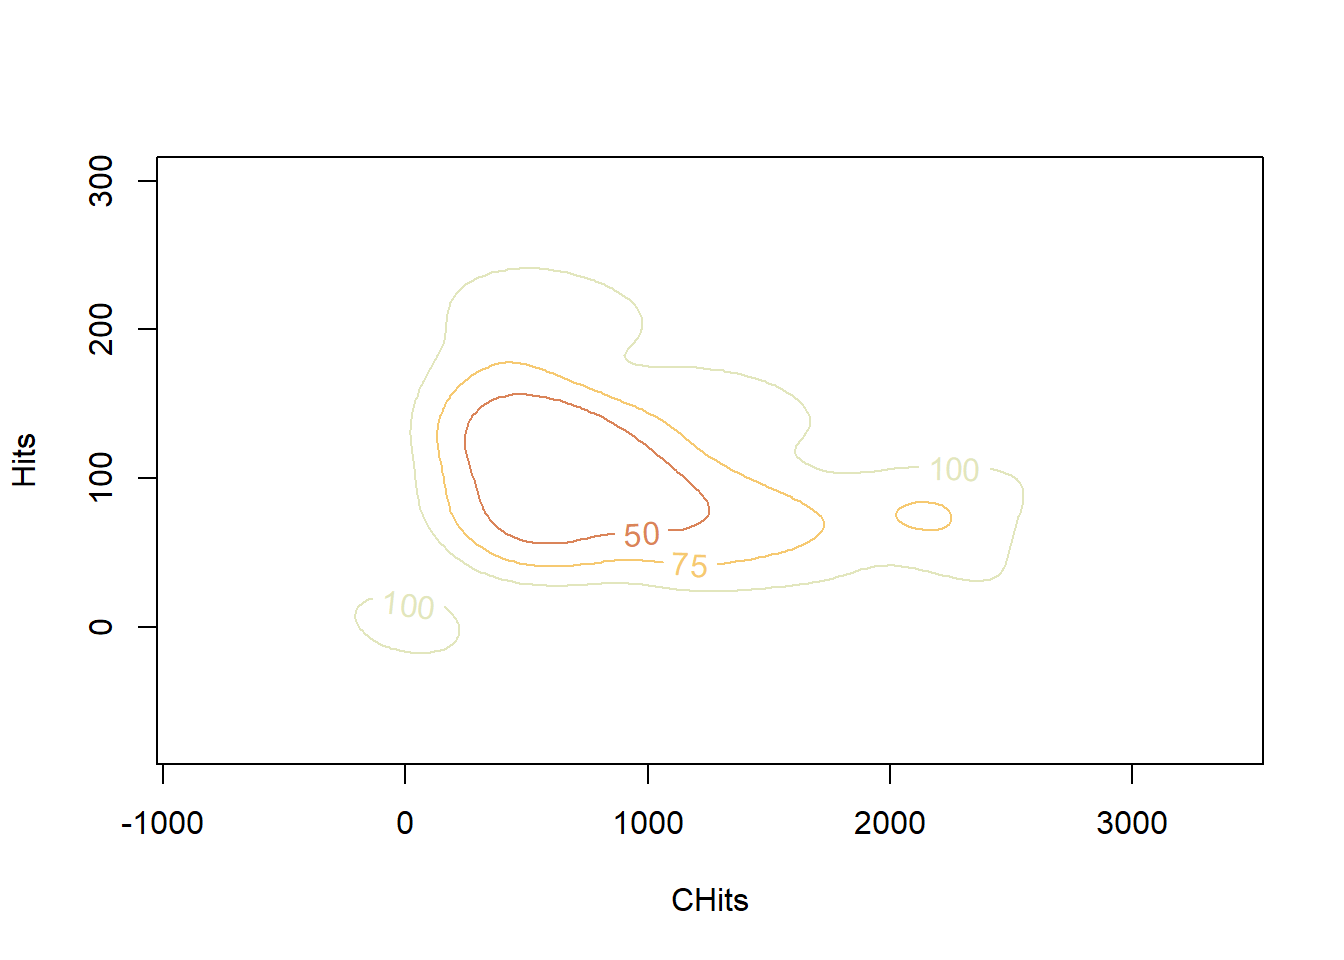
\includegraphics[scale=0.65]{Kernel.png}
    \end{figure}
    从图中可以看出,出错点在 CHits 和 Hits 上覆盖的范围比较广,而且形状不连续,
    另外模型本身的预测准确度已经不低,由此认为预测出错的原因很可能是出现离群值。
\end{document}